%%%%%%%%%%%%%%%%%%%%%%%%%%%%%%%%%%%%%%%%%
% Programming/Coding Assignment
% LaTeX Template
%
% This template has been downloaded from:
% http://www.latextemplates.com
%
% Original author:
% Ted Pavlic (http://www.tedpavlic.com)
%
% Note:
% The \lipsum[#] commands throughout this template generate dummy text
% to fill the template out. These commands should all be removed when
% writing assignment content.
%
% This template uses a Perl script as an example snippet of code, most other
% languages are also usable. Configure them in the "CODE INCLUSION
% CONFIGURATION" section.
%
%%%%%%%%%%%%%%%%%%%%%%%%%%%%%%%%%%%%%%%%%

%----------------------------------------------------------------------------------------
%    PACKAGES AND OTHER DOCUMENT CONFIGURATIONS
%----------------------------------------------------------------------------------------

\documentclass{article}

\usepackage{fancyhdr} % Required for custom headers
\usepackage{lastpage} % Required to determine the last page for the footer
\usepackage{extramarks} % Required for headers and footers
\usepackage[usenames,dvipsnames]{color} % Required for custom colors
\usepackage{graphicx} % Required to insert images
\usepackage{listings} % Required for insertion of code
\usepackage{courier} % Required for the courier font
\usepackage{lipsum} % Used for inserting dummy 'Lorem ipsum' text into the template
\usepackage[utf8]{inputenc}
\usepackage{amsmath,amssymb,amsfonts,amsthm,graphicx,enumitem}
\usepackage[parfill]{parskip}
\usepackage{color}
\usepackage{float}
\usepackage[ruled,linesnumbered]{algorithm2e}
\newcommand\mycommfont[1]{\footnotesize\ttfamily\textcolor{blue}{#1}}
\SetCommentSty{mycommfont}
% Margins
\topmargin=-0.45in
\evensidemargin=0in
\oddsidemargin=0in
\textwidth=6.5in
\textheight=9.0in
\headsep=0.25in

\linespread{1.1} % Line spacing

% Set up the header and footer
\pagestyle{fancy}
\lhead{\hmwkAuthorName} % Top left header
\chead{\hmwkClass\ (\hmwkClassInstructor\ \hmwkClassTime): \hmwkTitle} % Top center head
\rhead{\firstxmark} % Top right header
\lfoot{\lastxmark} % Bottom left footer
\cfoot{} % Bottom center footer
\rfoot{Page\ \thepage\ of\ \protect\pageref{LastPage}} % Bottom right footer
\renewcommand\headrulewidth{0.4pt} % Size of the header rule
\renewcommand\footrulewidth{0.4pt} % Size of the footer rule

\setlength\parindent{0pt} % Removes all indentation from paragraphs

%----------------------------------------------------------------------------------------
%    CODE INCLUSION CONFIGURATION
%----------------------------------------------------------------------------------------

\definecolor{MyDarkGreen}{rgb}{0.0,0.4,0.0} % This is the color used for comments
\lstloadlanguages{Perl} % Load Perl syntax for listings, for a list of other languages supported see: ftp://ftp.tex.ac.uk/tex-archive/macros/latex/contrib/listings/listings.pdf
\lstset{language=Perl, % Use Perl in this example
        frame=single, % Single frame around code
        basicstyle=\small\ttfamily, % Use small true type font
        keywordstyle=[1]\color{Blue}\bf, % Perl functions bold and blue
        keywordstyle=[2]\color{Purple}, % Perl function arguments purple
        keywordstyle=[3]\color{Blue}\underbar, % Custom functions underlined and blue
        identifierstyle=, % Nothing special about identifiers
        commentstyle=\usefont{T1}{pcr}{m}{sl}\color{MyDarkGreen}\small, % Comments small dark green courier font
        stringstyle=\color{Purple}, % Strings are purple
        showstringspaces=false, % Don't put marks in string spaces
        tabsize=5, % 5 spaces per tab
        %
        % Put standard Perl functions not included in the default language here
        morekeywords={rand},
        %
        % Put Perl function parameters here
        morekeywords=[2]{on, off, interp},
        %
        % Put user defined functions here
        morekeywords=[3]{test},
           %
        morecomment=[l][\color{Blue}]{...}, % Line continuation (...) like blue comment
        numbers=left, % Line numbers on left
        firstnumber=1, % Line numbers start with line 1
        numberstyle=\tiny\color{Blue}, % Line numbers are blue and small
        stepnumber=5 % Line numbers go in steps of 5
}

% Creates a new command to include a perl script, the first parameter is the filename of the script (without .pl), the second parameter is the caption
\newcommand{\perlscript}[2]{
\begin{itemize}
\item[]\lstinputlisting[caption=#2,label=#1]{#1.pl}
\end{itemize}
}

%----------------------------------------------------------------------------------------
%    DOCUMENT STRUCTURE COMMANDS
%    Skip this unless you know what you're doing
%----------------------------------------------------------------------------------------

% Header and footer for when a page split occurs within a problem environment
\newcommand{\enterProblemHeader}[1]{
\nobreak\extramarks{#1}{#1 continued on next page\ldots}\nobreak
\nobreak\extramarks{#1 (continued)}{#1 continued on next page\ldots}\nobreak
}

% Header and footer for when a page split occurs between problem environments
\newcommand{\exitProblemHeader}[1]{
\nobreak\extramarks{#1 (continued)}{#1 continued on next page\ldots}\nobreak
\nobreak\extramarks{#1}{}\nobreak
}

\setcounter{secnumdepth}{0} % Removes default section numbers
\newcounter{homeworkProblemCounter} % Creates a counter to keep track of the number of problems

\newcommand{\homeworkProblemName}{}
\newenvironment{homeworkProblem}[1][Problem \arabic{homeworkProblemCounter}]{ % Makes a new environment called homeworkProblem which takes 1 argument (custom name) but the default is "Problem #"
\stepcounter{homeworkProblemCounter} % Increase counter for number of problems
\renewcommand{\homeworkProblemName}{#1} % Assign \homeworkProblemName the name of the problem
\section{\homeworkProblemName} % Make a section in the document with the custom problem count
\enterProblemHeader{\homeworkProblemName} % Header and footer within the environment
}{
\exitProblemHeader{\homeworkProblemName} % Header and footer after the environment
}

\newcommand{\problemAnswer}[1]{ % Defines the problem answer command with the content as the only argument
\noindent\framebox[\columnwidth][c]{\begin{minipage}{0.98\columnwidth}#1\end{minipage}} % Makes the box around the problem answer and puts the content inside
}

\newcommand{\homeworkSectionName}{}
\newenvironment{homeworkSection}[1]{ % New environment for sections within homework problems, takes 1 argument - the name of the section
\renewcommand{\homeworkSectionName}{#1} % Assign \homeworkSectionName to the name of the section from the environment argument
\subsection{\homeworkSectionName} % Make a subsection with the custom name of the subsection
\enterProblemHeader{\homeworkProblemName\ [\homeworkSectionName]} % Header and footer within the environment
}{
\enterProblemHeader{\homeworkProblemName} % Header and footer after the environment
}

%----------------------------------------------------------------------------------------
%    NAME AND CLASS SECTION
%----------------------------------------------------------------------------------------

\newcommand{\hmwkTitle}{Mid-term} % Assignment title
\newcommand{\hmwkDueDate}{} % Due date
\newcommand{\hmwkClass}{Computer vision } % Course/class
\newcommand{\hmwkClassTime}{11:00am} % Class/lecture time
\newcommand{\hmwkClassInstructor}{Dr. Xiu Wen Liu} % Teacher/lecturer
\newcommand{\hmwkAuthorName}{Jian Wang } % Your name

%----------------------------------------------------------------------------------------
%    TITLE PAGE
%----------------------------------------------------------------------------------------

\title{
\vspace{2in}
\textmd{\textbf{\hmwkClass:\ \hmwkTitle}}\\
\normalsize\vspace{0.1in}\small{Due\ on\ \hmwkDueDate}\\
\vspace{0.1in}\large{\textit{\hmwkClassInstructor\ \hmwkClassTime}}
\vspace{3in}
}

\author{\textbf{\hmwkAuthorName}}
\date{} % Insert date here if you want it to appear below your name

%----------------------------------------------------------------------------------------

\begin{document}

\maketitle

%----------------------------------------------------------------------------------------
%    TABLE OF CONTENTS
%----------------------------------------------------------------------------------------

%\setcounter{tocdepth}{1} % Uncomment this line if you don't want subsections listed in the ToC

\newpage
\tableofcontents
\newpage

%% insert the programming code
%\begin{homeworkProblem}
%Listing \ref{homework_example} shows a Perl script.
%
%\perlscript{homework_example}{Sample Perl Script With Highlighting}
%
%\lipsum[1]
%\end{homeworkProblem}

%% insert the chart
%\begin{homeworkProblem}
%\lipsum[2]
%
%\problemAnswer{
%\begin{center}
%\includegraphics[width=0.75\columnwidth]{example_figure} % Example image
%\end{center}
%\lipsum[3-5]
%}
%\end{homeworkProblem}
%% Example of list array and emurate
%\begin{homeworkProblem}
%
%\begin{flalign}
%A =
%\begin{bmatrix}
%A_{11} & A_{21} \\
%A_{21} & A_{22}
%\end{bmatrix}
%\end{flalign}
%
%\begin{itemize}
%    \item First item in a list
%        \begin{itemize}
%        \item First item in a list
%            \begin{itemize}
%            \item First item in a list
%            \item Second item in a list
%            \end{itemize}
%        \item Second item in a list
%        \end{itemize}
%    \item Second item in a list
%\end{itemize}
%
%\begin{enumerate}
%\item First item in a list
%\item Second item in a list
%\item Third item in a list
%\end{enumerate}

%% equation formula
%$\left \{
%\begin{tabular}{l}
%$V_t+\frac{\sigma^2S^2}{2}V_{SS}+rSV_s - rV=0$\\
%
%$V(0,t)=e^{-r(T-t)}$\\
%
%$V(\infty,t)=0$\\
%
%$V(S,T)=I_{\{S\leq K\}}$
%\end{tabular}
%\right.$

%\end{homeworkProblem}
%----------------------------------------------------------------------------------------

% example of algorithm
%\begin{algorithm}
%\DontPrintSemicolon
%\Begin{
%$x \longleftarrow x_0$\\
%\For{k = 1 to maxiter}{
%$rmax \longleftarrow 0$\\
%\For {j = 1 to N-1}
%{ $r= y_j- (l_j x_{j-1}+d_jx_j+u_jx_{j+1})$\\
%  $x_{test}=x_j+\omega r /d_j$\\
%  \If{$x_{test}>payoff_j$}{
%      $x_j=x_{test}$\\
%      $rmax=max(rmax,|r|)$}
%  \Else
% {$x_j=payoff_j$}
% 
% \If{$r_{max}<Tol$}
% {exit}
% }
%}
%}
%\caption{PSOR Algoithm\label{IR}}
%\end{algorithm}

% example of table
%\begin{tabular}{|c|c|c|c|c|c|c|c|}
%\hline
%$N_x$&$N_t$&Backward&Rate& Crank Nicolson& Rate&Ranacher Smooth&Rate\\
%\hline
%20&    20&    0.317074957&&        0.314437672&&        0.322944148&    \\
%40&    40&    0.150341433&    2.11&     0.148175535&    2.12&     0.151402278&    2.13\\
%80&    80&    0.069756168&    2.16&     0.0693145&    2.14&     0.070194038&    2.16\\
%160&    160&    0.034760674&    2.01&     0.034475478&    2.01&     0.035016767&    2.00\\
%320&    320&    0.017298542&    2.01&     0.017207956&    2.00&     0.017418478&    2.01\\
%640&    640&    0.008643274&    2.00&     0.008598123&    2.00&     0.00869713&    2.00\\
%\hline
%\end{tabular}

%example of graph
%$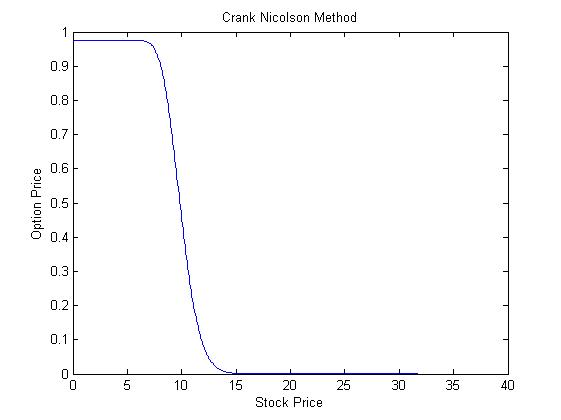
\includegraphics[height=3.5in,width=5in]{binary_option_price_cn.jpg}$\\
\section*{[Purpose]}
This mid-term project helps us to review the knowledge that we learned from the computer vision class.



\section*{[Problems]}
\textbf{Problem 1:}\\
1) describe how SIFT features are detected and how SIFT descriptors are computed. On typical images, how would you characterized the local patches centered at identified SIFT features in terms of the eigenvalues of the autocorrelation matrices? Briefly explain.\\
\textbf{Solution:} 
a) To compute SIFT features, first we need to compute the difference of Gaussian images. Then we detect local extreme by comparing each pixel by its eight neighborhoods in the same scale and nie neighbors in the scale above and below. Last step is to compute the descriptor s we first compute the gradient magnitude and orientation at each sample point around feature point. Then the samples are accumulated into orientation, histograms. Summarizing the contents over 4x4 subregions. Each oriental histogram has 8 bins for 8 directions. b) If the patch has two large eigenvalues, it represents a vertex. If it has one large eigenvalue, it is an edge. Otherwise, it is not a feature point.\\

2) In our version of the agglomerative hierarchical clustering algorithm, we sue the single-link as the between- clusters distances in the odd steps(2,4, and so on ) Show the step-by-step clustering results on the pairwise distances given on the following. In each step, you need to show which clusters are merged and what is the distance between the merged clusters. \\

\begin{bmatrix}
   .000&.480&.658&.456&.642&.183\\
   .480&.000&.425&.117&.391&.485\\
   .658&.425&.00&.418&.161&.644\\
   .456&.117&.418&.000&.382&.464\\
   .642&.391&.161&.382&.000&.607\\
   .183&.485&.644&.464&.607&.000\\
\end{bmatrix}
\\\\
\textbf{Solution:}\\
In \textit{single-link} clustering or \textit{single-linkage} clustering, the similarity of two clusters is the similarity of their most similar member. In \textit{completed-link} clustering or \textit{complete-linkage} clustering, the similarity is the similarity of the most dissimilar members.\\
Step 1: we use the single-link method, sample 2 and sample 4 are merged, the distance is =.117\\
Step 2: We use the complete-link method,  note here, we should use the \textbf{maximum} distance between the cluster \{2,4\} and other samples. for example, the distance between sample 1 and cluster \{2,4\} should be 0.480 instead of 0.456. In this step , sample 3 and sample 5 are merged , the distance is 0.161.\\
Step 3: use \textit{single-link},sample 1 and sample 6 are merged, the distance is 0.183.\\
Step 4: use \textit {completed-link},sample (2,4) and (3,5) are merged, the distance is 0.425.\\
Step 5: use \textit{single-link} sample(2,3,4,5) and (1,6) are merged.

3) Given the following image(on the left side), compute its histogram, assuming that a bin's range is [x-0.5,x+0.5], where x is the value at the center of the bin. Suppose that the pixel values must be between 0 and 7 inclusively, given an image with the same dimension (as the given image) so that the histogram intersection between the histograms of the two images is the smallest. You need to briefly explain your answer.\\

\begin{tabular}{|c|c|c|c|c|}
\hline
2 & 5 & 2 & 0 & 7\\
\hline
4 & 6 & 6 & 0 & 1\\
\hline
3 & 2 & 7 & 6 & 5\\
\hline
1 & 0 & 4 & 0 & 7\\
\hline
\end{tabular}

\textbf{Solution:} \\
\begin{center}
\begin{tabular}{|c|c|}
\hline
Pixel value & Numbers \\
\hline
[0, 1) & 3 \\
\hline
[1,2) & 2 \\
\hline
[2,3)& 3\\
\hline
[3,4)& 1\\
\hline
[4,5)& 3\\
\hline
[5,6)& 2\\
\hline
[6,7)& 6\\
\hline
\end{tabular}
\end{center}
The histogram of the image is given by the following chart:\\
\begin{center}
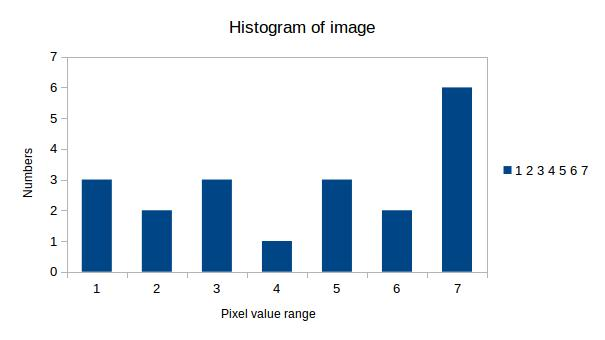
\includegraphics[width=0.75\columnwidth]{histogram-problem2} % Example image
\end{center}

4)W use the Canny edge detector to detect edges in an image. At pixel (x=150,y=200), $\frac{\partial f}{\partial x}$ is estimated to be -120 and $\frac{\partial f}{\partial y}$ is estimated to be 80; for non-maximum suppression, which two pixels shall be used for comparison at the given pixel? Justify your answer. We assume that the eight nearest neighbors are used.\\
\textbf{Solution:}\\
Since $(\frac{\partial f}{\partial x},\frac{\partial f}{\partial y})=(-120,80)$, so the derivation of gradient can be estimated by $\beta=arctan(-\frac{2}{3})\approx146.31^{o}$, which is rounded to $135^{o}$. Hence we compare it with the upper left and the lower right pixel.\\

5) Given the Laplacian pyramid(accuracy to three decimal digits) for the following image. Here we simply use the average value of involved pixels for down sampling and repeat the pixel value for up sampling, and we assume that the coarsest level has only a single pixel.\\
\textbf{Solution:}\\


\textbf{Problem 2} To train a real-time face detector, there are 8 face training images and 12 non-face training images, In the process of selecting the first optimal weak classifier, for a particular Haar feature, its values for all the face training images are 0.48,0.67,0.60,0.64,0.64,0.88,0.74,0.35 and its values for all the non-face training images are -0.09,0.31,0.15,0.38,0.27,0.45,0.10,0.28,0.29,0.37,0.58,0.15.Answer the following questions:\\

1) A common way to implement a face detector is to use a classifier to classify each local window whether it is a face. Explain the key differences of the real-time face detection method that enables it to achieve real-time detection compared to the common way.\\
Answer:\\
The real-time face detector contains the following key components:\\
a) A new image representation:The features can be computed fast and in constant time regardless of the scales\\
b)A simple and efficient (but also effective) classifier:Based on AdaBoost for feature selection and learning classifiers\\
c)Cascade of classifiers to reduce the average detection time for an image:A degenerated decision tree; often known as the twenty-question approach

2) Describe clearly how to efficiently compute the optimal weak classifier for this feature. Then plot the weighted error against the threshold for this feature and give ALL the parameters for the resulting optimal weaker classier.\\
Answer:\\
The algorithm to efficiently compute the optimal weak classifier is described in algorithm \ref{alg:ada}.


\begin{algorithm}
\DontPrintSemicolon
Given training example images:$(x_1,y_1),\dots,(x_n,y_n)$ \tcp*{assume two dimensions}
\ \ \ \ where $y_i=0,1$ for negative and positive examples respectively.\;
Initialize weights $w_{1,i}=\frac{1}{2m},\frac{1}{2l}$ for negative and positive training example respectively.\;

\ \ \ \ where m and l are the number of negatives and positives respectively\;
\For {$t=1,\dots,T$ }
{
Normailize weights so that $w_t$ is a distribution\;
For each feature j train a classifier $h_j$ and evaluate its error $\epsilon_j$ with respect to $w_t$\;
Chose the classifier $h_j$ with lowest error\;
Update weights according to : \;
$w_{t+1,j}=w_{t,j}\beta_{t}$
where $e_i=0$ is $x_i$ is classified correctly, 1 otherwise, and $\beta_t=\frac{\epsilon_t}{1-\epsilon_t}$
}
The final strong classifier is: \;
$h(x)=\left \{
\begin{tabular}{ll}
1&$\sum_{t=1}^{T}\alpha_t h_t(x)>=\frac{1}{2}\sum_{t=1}^{T}\alpha_t,where\ \alpha_t-log(\frac{1}{\beta_t})$\\

0 & otherwise\\
\end{tabular}
\right.$

\caption{AdaBoost for feature selection\label{alg:ada}}
\end{algorithm}
For each weak classifier is determined by a threshold and sign \;
$h(x,f,p,\theta)=\left \{
\begin{tabular}{ll}
1&if $pf(x)<p\theta$\\

0 & otherwise\\
\end{tabular}
\right.$
So the problem is how to find the best threshold for the criterion used in AdaBoost. To make this process in a fast way, we can use the following algorithm \ref{alg:threshold}\\
\begin{algorithm}
Training samples are sorted based on the current feature.\;
Optimal threshold is computed in a single pass over list.\;
Four sums are maintained and evaluated:\;
\ \ \ \ 1)The total sum of positive example weights $T^+$\\
\ \ \ \ 2)The total sum of negative example weights $T^-$\\
\ \ \ \ 3)The sum of positive weights below the current example $S^+$\\
\ \ \ \ 4)The sum of negative weights below the current example $S^-$\\
The error for a threshold which splits the range between the current and previous example in the sorted list.\\
$$e=min(S^++(T^--S^-),S^-+(T^+-S^+)) $$
\caption{How to choose threshold\label{alg:threshold}}
\end{algorithm}

In this problem, we let the weights for positive sample as 1/2*8=1/16 and the weights for negative numbers as 1/2*12=1/24. \\
Now change the threshold and calculate the different sum of weights to find the error. \\
After we sort the list, it becomes $- - - - - - - - + - - - + - + + + + + +$, if we put the threshold between the first and the second element, $- | - - - - - - - + - - - + - + + + + + +$, the $T^+$ is 0.5 and the $T^-$ is also 0.5,the $S^+$ is 0, and the $S^-$ is 1/24, so the error for the threshold is:$ e=min(S^++(T^--S^-),S^-+(T^+-S^+))=min(11/24,13/24)=11/24.$,
similarly, the error for the threshold between the second and the third element is:10/24,9/24,8/24,7/24,6/24,5/24,4/24,11/48,9/48,7/48,5/48,8/48,6/48,9/48,
12/48,15/48,18/48. The minimum threshold is 5/48, which occurs between 0.45 and 0.48, so we can choose the threshold 0.465.\\

3)Suppose that this Haar feature gives the lowest weighted error among all the haar features, what are the weights used to choose the second optimal weak classifier? You need to specify the weight for each sample.\\
Answer: if we take threshold as 0.465, the sample bigger than this threshold will be classified as 1, and -1 vice versa. Only two samples are misclassified,  the 9th sample(positive misclassified as negative) and the 14th(negative misclassified as positive) sample. So we only need to change the weights of these two samples and leave others unchanged.




\end{document} 